\documentclass{article}
\usepackage[T1]{fontenc}
\usepackage{lmodern}
\usepackage{graphicx}
\usepackage{amsmath,amssymb}
\usepackage[a4paper,margin=2cm]{geometry}
\usepackage[absolute,overlay]{textpos}
\setlength{\TPHorizModule}{1mm}
\setlength{\TPVertModule}{1mm}
\usepackage[indonesian]{babel}
\usepackage{hyperref}
\setlength{\emergencystretch}{2em}
% unit: Halaman 108

\begin{document}

% === Halaman 108 (llm) ===

\vspace{242.05mm}

\section*{E. Enigma Cipher}

\begin{itemize}
    \item Enigma adalah mesin enkripsi elektromekanik untuk melakukan enkripsi dan dekripsi.
    \item Ditemukan dan dipatenkan oleh insinyur Jerman, Arthur Scherbius, untuk tujuan komersil, diplomatik, dan militer
    \item Menjadi terkenal karena digunakan oleh tantara Nazi Jerman selama Perang Dunia II untuk mengenkripsi/dekripsi pesan-pesan militer.
    \item Enigma berasal dari bahasa latin, \textit{enigmae}, yang artinya teka-teki.
\end{itemize}

% deskripsi: Foto mesin Enigma dengan label keterangan bagian-bagiannya seperti Rotors, Keyboard, Lampboard, dan Plugboard.
% bbox normalisasi: [0.5760, 0.0700, 0.9370, 0.8850]
\begin{textblock*}{75.81mm}(120.96mm,20.79mm)
\noindent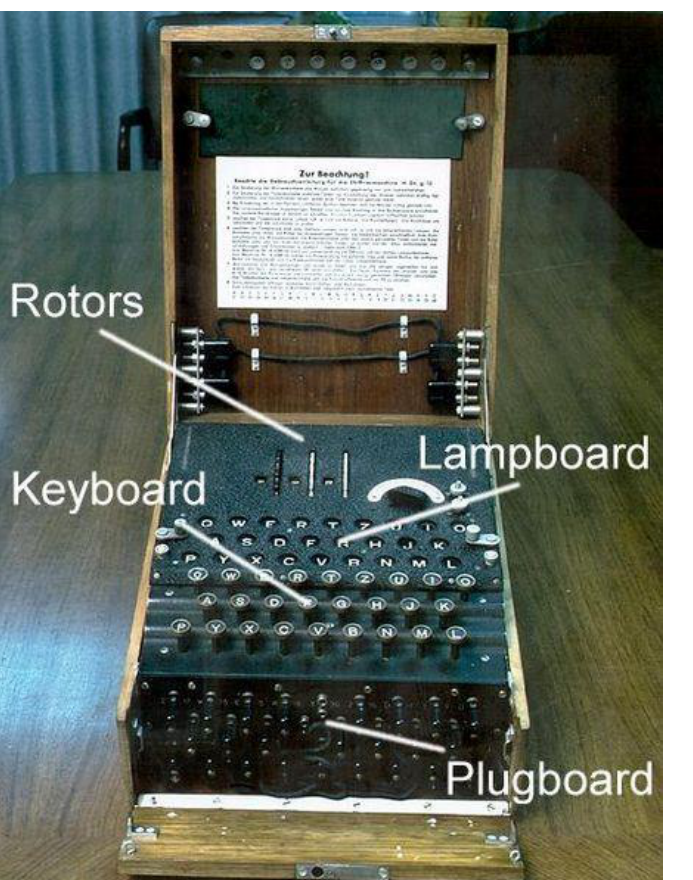
\includegraphics[width=75.81mm,height=242.05mm]{../../images/llm/page_108_img_01.png}%
\end{textblock*}

\end{document}
